\chapter{Perancangan}
\label{chap:perancangan}

Pada bab ini akan dijelaskan mengenai perancangan Sistem Informasi Riwayat
Mahasiswa yang akan dibuat. Mulai dari perancangan tampilan {\it web} yang digunakan,
perancangan modul, dan perancangan diagram sekuens.

\section{Perancangan Tampilan {\it Web} Yang Digunakan}
\label{sec:perancanganantarmuka}

Perancangan tampilan {\it web} yang akan dibuat untuk mengimplementasikan Sistem
Informasi Riwayat Mahasiswa terdapat tujuh buah perancangan yaitu halaman
awal, pilih mahasiswa, info mahasiswa, edit mahasiswa, lihat histori, lihat
versi ini dan entri baru.

\subsection{Tampilan Halaman Awal}
Perancangan tampilan {\it web} untuk halaman utama dapat dilihat pada
Gambar~\ref{fig:halamanawal}.

\begin{figure}[ht]
\centering
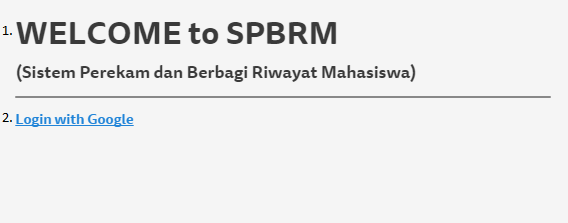
\includegraphics[scale=0.9]{Gambar/halamanawal.png}
\caption[Desain Antarmuka Halaman Awal]{Desain Antarmuka Halaman Awal}
\label{fig:halamanawal}
\end{figure}

Keterangan :
\begin{enumerate}[(1)]
\item
Bagian ini merupakan judul halaman awal perangkat lunak dan terdapat keterangan dari SPBRM.
\item
Bagian ini merupakan {\it link} berupa teks yang dapat diklik untuk melakukan login dengan menggunakan akun Google.
\end{enumerate}

\subsection{Tampilan {\it Web} Pilih Mahasiswa}
Perancangan tampilan {\it web} untuk pilih mahasiswa dapat dilihat pada
Gambar~\ref{fig:pilihmahasiswa}.

\begin{figure}[ht]
\centering
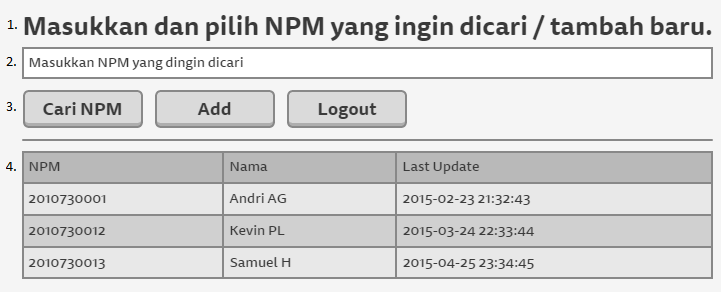
\includegraphics[scale=0.8]{Gambar/pilihmahasiswa.png}
\caption[Desain Antarmuka Pilih Mahasiswa]{Desain Antarmuka Pilih Mahasiswa}
\label{fig:pilihmahasiswa}
\end{figure}

Keterangan :
\begin{enumerate}[(1)]
\item
Bagian ini merupakan judul dari halaman untuk memilih mahasiswa.
\item
Bagian ini merupakan area untuk memasukkan npm yang ingin dicari oleh pengguna.
\item
Bagian ini merupakan tombol untuk melakukan aksi cari npm, add maupun logout.
\item
Bagian ini merupakan tempat menampilkan data mahasiswa dalam bentuk tabel. NPM dapat diklik oleh pengguna untuk memilih mahasiswa.
\end{enumerate}

\subsection{Tampilan {\it Web} Cari Mahasiswa}
Perancangan tampilan {\it web} untuk pilih mahasiswa dapat dilihat pada
Gambar~\ref{fig:carimahasiswa}.

\begin{figure}[ht]
\centering
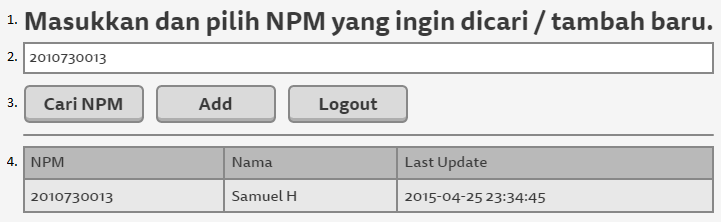
\includegraphics[scale=0.8]{Gambar/carimahasiswa.png}
\caption[Desain Antarmuka Cari Mahasiswa]{Desain Antarmuka Cari Mahasiswa}
\label{fig:carimahasiswa}
\end{figure}

Keterangan :
\begin{enumerate}[(1)]
\item
Bagian ini merupakan judul dari halaman untuk mencari mahasiswa.
\item
Bagian ini merupakan area untuk memasukkan npm yang ingin dicari oleh pengguna.
\item
Bagian ini merupakan tombol untuk melakukan aksi add atau logout.
\item
Bagian ini merupakan tempat menampilkan data mahasiswa yang dicari oleh pengguna dalam bentuk tabel. NPM dapat diklik oleh pengguna untuk memilih mahasiswa.
\end{enumerate}

\subsection{Tampilan {\it Web} Info Mahasiswa}
Perancangan tampilan {\it web} untuk info mahasiswa dapat dilihat pada Gambar~\ref{fig:infomahasiswa}.
\begin{figure}[ht]
\centering
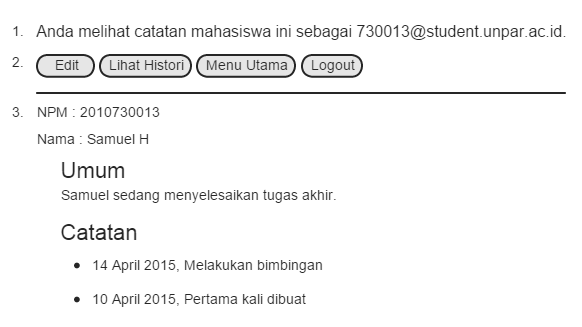
\includegraphics[scale=0.8]{Gambar/infomahasiswa.png}
\caption[Desain Antarmuka Info Mahasiswa]{Desain Antarmuka Info Mahasiswa}
\label{fig:infomahasiswa}
\end{figure}

Keterangan :
\begin{enumerate}[(1)]
\item
Bagian ini merupakan judul dari halaman info mahasiswa yang menampilkan keterangan pengguna yang sedang mengakses atau melihat info mahasiswa tersebut.
\item
Bagian ini merupakan tombol untuk melakukan aksi pindah ke menu utama, mengedit, membuat catatan masalah baru, lihat daftar masalah, lihat histori dan logout.
\item
Bagian ini merupakan tempat menampilkan info mahasiswa berupa npm, nama, deskripsi umum dan catatan yang berasal dari {\it databasse}.
\end{enumerate}

\subsection{Tampilan {\it Web} Edit Info Mahasiswa}
Perancangan tampilan {\it web} untuk edit info mahasiswa dapat dilihat pada Gambar~\ref{fig:editmahasiswa}.
\begin{figure}[ht]
\centering
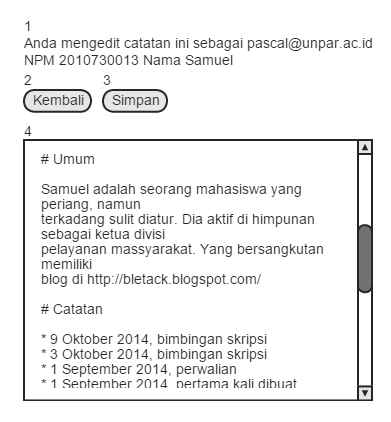
\includegraphics[scale=0.8]{Gambar/editmahasiswa.png}
\caption[Desain Antarmuka Edit Info Mahasiswa]{Desain Antarmuka Edit Info Mahasiswa}
\label{fig:editmahasiswa}
\end{figure}

Keterangan :
\begin{enumerate}[(1)]
\item
Bagian ini merupakan judul dari halaman edit info mahasiswa yang menampilkan keterangan pengguna yang sedang mengedit info mahasiswa tersebut.
\item
Bagian ini merupakan teks yang menampilkan NPM dan nama mahasiswa yang telah dipilih oleh pengguna untuk diedit infonya.
\item
Bagian ini merupakan tombol untuk melakukan aksi kembali ke info mahasiswa, simpan untuk perubahan yang telah dilakukan, pindah ke menu utama, dan logout.
\item
Bagian ini merupakan teks yang merupakan bagian untuk mengedit deskripsi umum.
\item
Bagian ini merupakan tempat yang menampilkan deskripsi umum seorang mahasiswa yang telah dipilih oleh pengguna. Deskripsi umum yang ditampilkan pada bagian ini berasal dari {\it database} dan pengguna dapat melakukan perubahan pada deskripsi umum di bagian ini.
\item
Bagian ini merupakan teks yang merupakan bagian untuk mengedit catatan.
\item
Bagian ini merupakan tempat yang menampilkan catatan seorang mahasiswa yang telah dipilih oleh pengguna. Catatan yang ditampilkan pada bagian ini berasal dari {\it database} dan pengguna dapat melakukan perubahan pada catatan di bagian ini.
\end{enumerate}

\subsection{Tampilan {\it Web} Tambah Masalah Baru}
Perancangan tampilan {\it web} untuk info mahasiswa dapat dilihat pada Gambar~\ref{fig:masalahbaru}.
\begin{figure}[ht]
\centering
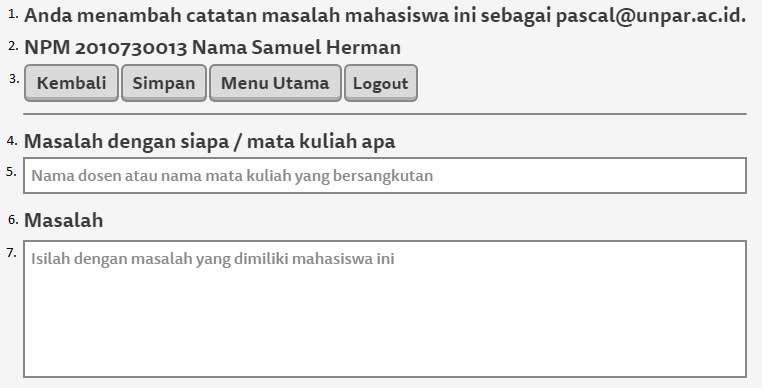
\includegraphics[scale=0.8]{Gambar/masalahbaru.png}
\caption[Desain Antarmuka Tambah Masalah Baru]{Desain Antarmuka Tambah Masalah Baru}
\label{fig:masalahbaru}
\end{figure}

Keterangan :
\begin{enumerate}[(1)]
\item
Bagian ini merupakan judul dari halaman tambah masalah baru yang menampilkan keterangan pengguna yang sedang menambah catatan masalah baru.
\item
Bagian ini merupakan teks yang menampilkan NPM dan nama mahasiswa yang telah dipilih oleh pengguna untuk ditambah catatan masalah.
\item
Bagian ini merupakan tombol untuk melakukan aksi kembali ke info mahasiswa, edit, pindah ke menu utama, dan logout.
\item
Bagian ini merupakan teks yang merupakan bagian masalah bersangkutan dengan siapa / mata kuliah apa.
\item
Bagian ini merupakan tempat untuk memasukkan pihak yang bersangkutan oleh pengguna. Pihak yang bersangkutan dapat diisi dengan nama dosen atau nama mata kuliah.
\item
Bagian ini merupakan teks yang merupakan bagian masalahnya.
\item
Bagian ini merupakan tempat untuk memasukkan penjelasan atau rincian masalah yang dimiliki mahasiswa tersebut oleh pengguna.
\end{enumerate}

\subsection{Tampilan {\it Web} Lihat Daftar Masalah}
Perancangan tampilan {\it web} untuk info mahasiswa dapat dilihat pada Gambar~\ref{fig:lihatmasalah}.
\begin{figure}[ht]
\centering
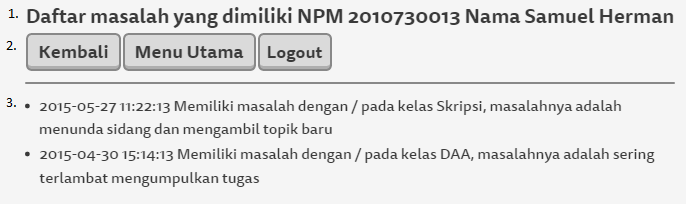
\includegraphics[scale=0.9]{Gambar/lihatmasalah.png}
\caption[Desain Antarmuka Lihat Daftar Masalah]{Desain Antarmuka Lihat Daftar Masalah}
\label{fig:lihatmasalah}
\end{figure}

Keterangan :
\begin{enumerate}[(1)]
\item
Bagian ini merupakan judul dari halaman lihat daftar masalah yang menampilkan keterangan npm dan nama dari mahasiswa yang dipilih oleh pengguna.
\item
Bagian ini merupakan tombol untuk melakukan aksi kembali ke info mahasiswa, pindah ke menu utama, dan logout.
\item
Bagian ini merupakan tempat menampilkan daftar masalah dari mahasiswa yang dipilih oleh pengguna. Daftar masalah tersebut berasal dari {\it database}.
\end{enumerate}

\subsection{Tampilan {\it Web} Lihat Histori}
Perancangan tampilan {\it web} untuk lihat histori dapat dilihat pada Gambar~\ref{fig:lihathistori}.
\begin{figure}[ht]
\centering
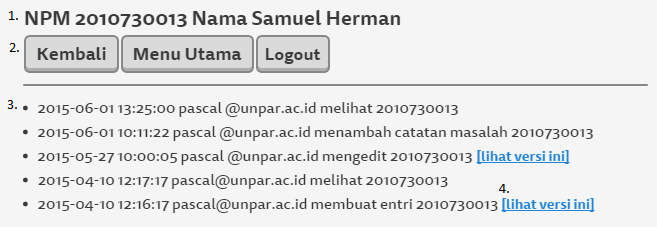
\includegraphics[scale=0.9]{Gambar/lihathistori.png}
\caption[Desain Antarmuka Lihat Histori]{Desain Antarmuka Lihat Histori}
\label{fig:lihathistori}
\end{figure}

Keterangan :
\begin{enumerate}[(1)]
\item
Bagian ini merupakan teks yang menampilkan keterangan NPM dan nama mahasiswa yang telah dipilih untuk dilihat historinya.
\item
Bagian ini merupakan tombol untuk melakukan aksi kembali ke info mahasiswa, pindah ke menu utama, dan logout.
\item
Bagian ini merupakan daftar histori dari mahasiswa yang telah dipilih. Daftar histori tersebut berasal dari {\it database}.
\item
Bagian ini merupakan {\it link} yang dapat digunakan pengguna untuk mengakses keterangan versi dari awal sampai yang terakhir.
\end{enumerate}

\subsection{Tampilan {\it Web} Lihat Versi Ini}
Perancangan tampilan {\it web} untuk lihat versi ini dapat dilihat pada
Gambar~\ref{fig:lihatversiini}.
\begin{figure}[ht]
\centering
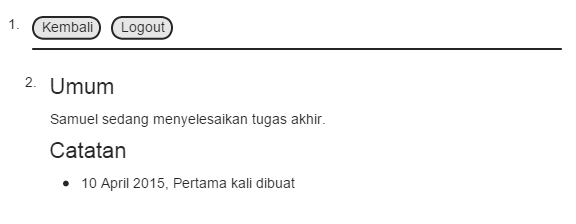
\includegraphics[scale=0.8]{Gambar/lihatversiini.png}
\caption[Desain Antarmuka Lihat Versi Ini]{Desain Antarmuka Lihat Versi Ini}
\label{fig:lihatversiini}
\end{figure}

Keterangan :
\begin{enumerate}[(1)]
\item
Bagian ini merupakan teks yang menampilkan keterangan pengguna yang membuat versi ini.
\item
Bagian ini merupakan tombol untuk melakukan aksi kembali ke lihat histori dan logout.	
\item
Bagian ini tempat menampilkan info dari mahasiswa yang telah dipilih. Info yang ditampilkan adalah deskripsi umum dan catatan. Info mahasiswa tersebut berasal dari {\it database}.
\end{enumerate}

\subsection{Tampilan {\it Web} Entri Baru}
Perancangan tampilan {\it web} untuk entri baru dapat dilihat pada Gambar~\ref{fig:entribaru}.
\begin{figure}[ht]
\centering
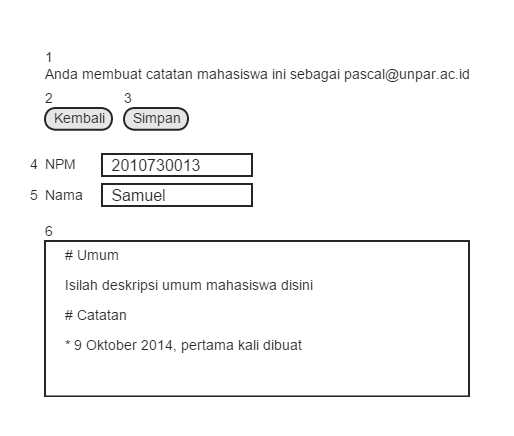
\includegraphics[scale=0.9]{Gambar/entribaru.png}
\caption[Desain Antarmuka Entri Baru]{Desain Antarmuka Entri Baru}
\label{fig:entribaru}
\end{figure}

Keterangan :
\begin{enumerate}[(1)]
\item
Bagian ini merupakan judul dari halaman entri baru yang menampilkan keterangan pengguna yang sedang menambah entri baru.
\item
Bagian ini merupakan tombol untuk melakukan aksi kembali ke pilih mahasiswa, simpan, pindah ke menu utama, dan logout.
\item
Bagian ini merupakan teks dan tempat untuk memasukkan npm seorang mahasiswa.
\item
Bagian ini merupakan teks dan tempat untuk memasukkan nama seorang mahasiswa.
\item
Bagian ini merupakan teks dan tempat untuk memasukkan deskripsi umum seorang mahasiswa.
\item
Bagian ini merupakan teks dan tempat untuk memasukkan catatan seorang mahasiswa.
\end{enumerate}

\section{Perancangan Modul}
\label{sec:perancanganmodul}

Perancangan modul untuk sistem informasi riwayat mahasiswa yang akan dibuat
dapat dilihat pada sub bab berikut.

\subsection{Modul Login}
Modul login yang dilakukan oleh pengguna (dosen) dapat dilihat pada Tabel
\ref{tab:modullogin}.

\begin{table}[ht]
\centering
\caption[Tabel Modul Login]{Modul Login}
\label{tab:modullogin}
\begin{tabular}{|c|p{10cm}|}
\hline
Nama Modul & index.php\\
\hline
Input & {\it username}, {\it password}\\
\hline
Output & -\\
\hline
Tabel yang diakses & -\\
\hline
Deskripsi & Pengguna memasukkan {\it username} dan {\it password} dari akun dosen (@unpar.ac.id) kemudian sistem akan melakukan autentikasi dan otorisasi menggunakan Google Oauth.\\
\hline
\end{tabular}
\end{table}

\subsection{Modul Pilih Mahasiswa}
Modul pilih mahasiswa yang dilakukan oleh pengguna (dosen) dapat dilihat pada
Tabel \ref{tab:modulpilihmahasiswa}.

\begin{table}[ht]
\centering
\caption[Tabel Modul Pilih Mahasiswa]{Modul Pilih Mahasiswa}
\label{tab:modulpilihmahasiswa}
\begin{tabular}{|c|p{10cm}|}
\hline
Nama Modul & list.php\\
\hline
Input & npm\\
\hline
Output & Tabel mahasiswa\\
\hline
Tabel yang diakses & InfoMahasiswa\\
\hline
Deskripsi & Pengguna memilih npm yang terdapat pada tabel untuk mahasiswa yang ingin dicari, kemudian dengan menekan npm yang terdapat pada tabel sebagai masukkan yang akan diteruskan ke modul info mahasiswa dan pengguna juga dapat membaut entri baru dengan menekan tombol ''{\it Add}''.\\
\hline
\end{tabular}
\end{table}

\subsection{Modul Cari Mahasiswa}
Modul cari mahasiswa yang dilakukan oleh pengguna (dosen) dapat dilihat pada Tabel \ref{tab:modulcarimahasiswa}.

\begin{table}[ht]
\centering
\caption[Tabel Modul Cari Mahasiswa]{Modul Cari Mahasiswa}
\label{tab:modulcarimahasiswa}
\begin{tabular}{|c|p{10cm}|}
\hline
Nama Modul & search.php\\
\hline
Input & npm\\
\hline
Output & Tabel mahasiswa\\
\hline
Tabel yang diakses & InfoMahasiswa\\
\hline
Deskripsi & Pengguna mencari npm yang ingin dicari dengan memasukkan npm pada tempat yang disediakan untuk memasukkan npm. Kemudian pengguna menekan tombol "Cari NPM" dan pengguna akan mendapatkan daftar mahasiswa sesuai dengan npm yang dimasukkan sebelumnya. Pengguna dapat menekan npm yang terdapat pada tabel sebagai masukkan yang akan diteruskan ke modul info mahasiswa dan pengguna juga dapat membaut entri baru dengan menekan tombol ''{\it Add}''.\\
\hline
\end{tabular}
\end{table}

\subsection{Modul Info Mahasiswa}
Modul info mahasiswa yang dilakukan oleh pengguna (dosen) dapat dilihat pada
Tabel \ref{tab:modulinfomahasiswa}.

\begin{table}[ht]
\centering
\caption[Tabel Modul Info Mahasiswa]{Modul Info Mahasiswa}
\label{tab:modulinfomahasiswa}
\begin{tabular}{|c|p{10cm}|}
\hline
Nama Modul & view.php\\
\hline
Input & -\\
\hline
Output & Info mahasiswa\\
\hline
Tabel yang diakses & InfoMahasiswa dan Histori\\
\hline
Deskripsi & Pengguna mendapatkan laporan barupa info mahasiswa yang telah dipilih sebelumnya pada modul pilih mahasiswa. Pengguna dapat melakukan enam aksi pada modul ini. Pertama, kembali ke halaman utama dengan menekan tombol "Menu Utama". Kedua, dapat merubah info mahasiswa yang ada dengan menekan tombol "{\it Edit}". Ketiga, dapat menambah catatan masalah baru dengan menekan tombol "Masalah Baru". Keempat, dapat melihat daftar masalah yang dimiliki mahasiswa tersebut dengan menekan tombol "Lihat Masalah". Kelima, dapat melihat histori mahasiswa tersebut dengan menekan tombol "Lihat Histori". Keenam, dapat keluar dari sistem dengan menekan tombol "{\it Logout}"\\
\hline
\end{tabular}
\end{table}

\subsection{Modul Edit Mahasiswa}
Modul {\it edit} mahasiswa yang dilakukan oleh pengguna (dosen) dapat dilihat
pada Tabel \ref{tab:moduleditmahasiswa}.

\begin{table}[ht]
\centering
\caption[Tabel Modul {\it Edit} Mahasiswa]{Modul {\it Edit} Mahasiswa}
\label{tab:moduleditmahasiswa}
\begin{tabular}{|c|p{10cm}|}
\hline
Nama Modul & edit.php\\
\hline
Input & teks\\
\hline
Output & -\\
\hline
Tabel yang diakses & InfoMahasiswa dan Histori\\
\hline
Deskripsi & Pengguna memasukkan atau merubah keterangan mahasiswa pada teks area lalu pengguna menyimpan dengan menekan tombol "Simpan" untuk menaruh perubahan yang dilakukan. Pengguna dapat kembali ke modul info mahasiswa tanpa melakukan perubahan dengan menekan tombol "Kembali".\\
\hline
\end{tabular}
\end{table}

\subsection{Modul Menambah Masalah Baru}
Modul menambah masalah baru yang dilakukan oleh pengguna (dosen) dapat dilihat pada Tabel \ref{tab:modulmasalahbaru}.

\begin{table}[ht]
\centering
\caption[Tabel Modul Menambah Masalah Baru]{Modul Menambah Masalah Baru}
\label{tab:modulmasalahbaru}
\begin{tabular}{|c|p{10cm}|}
\hline
Nama Modul & newproblem.php\\
\hline
Input & teks\\
\hline
Output & -\\
\hline
Tabel yang diakses & Masalah dan Histori\\
\hline
Deskripsi & Pengguna memasukkan pihak yang bersangkutan dan masalah yang dimiliki mahasiswa pada teks area yang telah disediakan lalu pengguna menyimpan catatan masalah tersebut dengan menekan tombol "Simpan". Pengguna dapat kembali ke modul info mahasiswa tanpa menambah catatan masalah dengan menekan tombol "Kembali".\\
\hline
\end{tabular}
\end{table}

\subsection{Modul Lihat Daftar Masalah}
Modul lihat daftar masalah yang dilakukan oleh pengguna (dosen) dapat dilihat pada Tabel \ref{tab:modullihatmasalah}.

\begin{table}[ht]
\centering
\caption[Tabel Modul Lihat Daftar Masalah]{Modul Lihat Daftar Masalah}
\label{tab:modullihatmasalah}
\begin{tabular}{|c|p{10cm}|}
\hline
Nama Modul & problem.php\\
\hline
Input & -\\
\hline
Output & Daftar masalah mahasiswa\\
\hline
Tabel yang diakses & Masalah\\
\hline
Deskripsi & Pengguna mendapatkan laporan berupa daftar masalah yang dimiliki seorang mahasiswa. Daftar masalah yang dapat dilihat antara lain pihak yang bersangkutan dengan masalah dan rincian / penjelasan masalah tersebut. Pengguna dapat kembali ke modul info mahasiswa dengan menekan tombol "Kembali".\\
\hline
\end{tabular}
\end{table}

\subsection{Modul Lihat Histori}
Modul lihat histori yang dilakukan oleh pengguna (dosen) dapat dilihat pada
Tabel \ref{tab:modullihathistori}.

\begin{table}[ht]
\centering
\caption[Tabel Modul Lihat Histori]{Modul Lihat Histori}
\label{tab:modullihathistori}
\begin{tabular}{|c|p{10cm}|}
\hline
Nama Modul & history.php\\
\hline
Input & -\\
\hline
Output & Daftar histori mahasiswa\\
\hline
Tabel yang diakses & Histori\\
\hline
Deskripsi & Pengguna mendapatkan laporan berupa daftar histori yang dimiliki setiap mahasiswa. Histori yang dapat dilihat antara lain aksi yang dilakukan pengguna baik aksi membuat entri, melihat dan mengedit. Kemudian berbagai versi keterangan yang dapat dilihat, mulai dari veri pertama kali dibuat hingga versi saat ini. Pengguna dapat kembali ke modul info mahasiswa dengan menekan tombol "Kembali".\\
\hline
\end{tabular}
\end{table}

\subsection{Modul Entri Baru}
Modul entri baru yang dilakukan oleh pengguna (dosen) dapat dilihat pada Tabel
\ref{tab:modulentribaru}.

\begin{table}[ht]
\centering
\caption[Tabel Modul Entri Baru]{Modul Entri Baru} 
\label{tab:modulentribaru}
\begin{tabular}{|c|p{10cm}|}
\hline
Nama Modul & new.php\\
\hline
Input & npm, nama, dan teks dalam format markdown\\
\hline
Output & -\\
\hline
Tabel yang diakses & InfoMahasiswa dan Histori\\
\hline
Deskripsi & Pengguna memasukkan npm, nama, deskripsi umum dan catatan mahasiswa pada teks area yang telah disediakan. Lalu pengguna menyimpan data-data yang telah dimasukkan dengan menekan tombol "Simpan" untuk membuat entri baru tersebut. Pengguna dapat kembali ke modul pilih mahasiswa tanpa melakukan perubahan dengan menekan tombol "Kembali".\\
\hline
\end{tabular}
\end{table}

\section{Perancangan Diagram Relasional}
\label{sec:perancangandiagramrelasional}

Berdasarkan ERD pada sub sub bab 3.6.3, maka dapat dihasilkan perancangan diagram relasional yang dapat dilihat pada Gambar \ref{fig:diagramrelasional}.

\begin{figure}[ht]
\centering
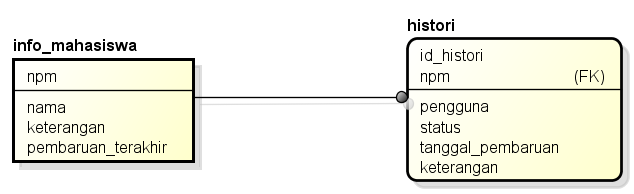
\includegraphics[scale=0.9]{Gambar/diagramrelasional.png}
\caption[Diagram Relasional]{Diagram Relasional} 
\label{fig:diagramrelasional}
\end{figure}

\section{Perancangan Tabel Sistem Perekam dan Berbagi Riwayat Mahasiswa}
\label{sec:perancangantabel}

\subsection{Perancangan Tabel Info Mahasiswa}
Untuk rancangan tabel info mahasiswa dapat dilihat pada Tabel
\ref{tab:rancangantabelinfomahasiswa}.

\begin{table}[ht]
\caption[Tabel Rancangan Tabel Info Mahasiswa]{Rancangan Tabel Info Mahasiswa}
\label{tab:rancangantabelinfomahasiswa}
\centering
\begin{tabular}{|l|l|p{1.2cm}|p{1.2cm}|p{1.2cm}|l|}
\hline
Atribut & Tipe Data & Ukuran & Primary Key & Foreign Key & Keterangan\\
\hline
npm & varchar & 10 & yes & no & -\\
\hline
nama & varchar & 60 & no & no & -\\
\hline
keterangan & text & - & no & no & -\\
\hline
catatan & text & - & no & no & -\\
\hline
pembaruan\_terakhir & datetime & - & no & no & -\\
\hline
\end{tabular}
\end{table}

\subsection{Perancangan Tabel Histori}
Untuk rancangan tabel histori dapat dilihat pada Tabel
\ref{tab:rancangantabelhistori}.

\begin{table}[ht]
\caption[Tabel Rancangan Tabel Histori]{Rancangan Tabel Histori}
\label{tab:rancangantabelhistori}
\centering
\begin{tabular}{|l|l|p{1.2cm}|p{1.2cm}|p{1.2cm}|l|}
\hline
Atribut & Tipe Data & Ukuran & Primary Key & Foreign Key & Keterangan\\
\hline
id\_histori & int & 5 & yes & no & AUTO\_INCREMENT\\
\hline
npm & varchar & 10 & no & yes & -\\
\hline
pengguna & varchar & 60 & no & no & -\\
\hline
status & text & - & no & no & -\\
\hline
tanggal\_pembaruan & datetime & - & no & no & -\\
\hline
keterangan & text & - & no & no & -\\
\hline
catatan & text & - & no & no & -\\
\hline
\end{tabular}
\end{table}

\subsection{Perancangan Tabel Masalah}
Untuk rancangan tabel masalah dapat dilihat pada Tabel
\ref{tab:rancangantabelmasalah}.

\begin{table}[ht]
\caption[Tabel Rancangan Tabel Masalah]{Rancangan Tabel Masalah}
\label{tab:rancangantabelmasalah}
\centering
\begin{tabular}{|l|l|p{1.2cm}|p{1.2cm}|p{1.2cm}|l|}
\hline
Atribut & Tipe Data & Ukuran & Primary Key & Foreign Key & Keterangan\\
\hline
id\_masalah & int & 5 & yes & no & AUTO\_INCREMENT\\
\hline
npm & varchar & 10 & no & yes & -\\
\hline
pengguna & varchar & 60 & no & no & -\\
\hline
masalah\_dengan & varchar & 25 & no & no & -\\
\hline
masalah & text & - & no & no & -\\
\hline
tanggal & datetime & - & no & no & -\\
\hline
\end{tabular}
\end{table}


%\section{Diagram Sekuens}
%\label{sec:diagramsekuens}

%Pembuatan diagram sekuens mengacu pada Gambar~\ref{fig:usecase}. Terdapat tiga diagram sekuens yaitu 
%\begin{enumerate}[(1)]
%  \item Sekuens bagian satu mencakup proses login dapat dilihat pada Gambar
%  \ref{fig:ds1}.
%  \item Sekuens bagian dua mencakup proses memilih mahasiswa, melihat   info mahasiswa, dan membuat entri baru. Dapat dilihat pada Gambar \ref{fig:ds2}.
%  \item Sekuens bagian tiga mencakup melihat info mahasiswa, mengedit info   mahasiswa, melihat histori, dan melihat keterangan versi ini. Dapat dilihat pada Gambar \ref{fig:ds3}.
%\end{enumerate}

%\begin{figure}[p]
%\centering
%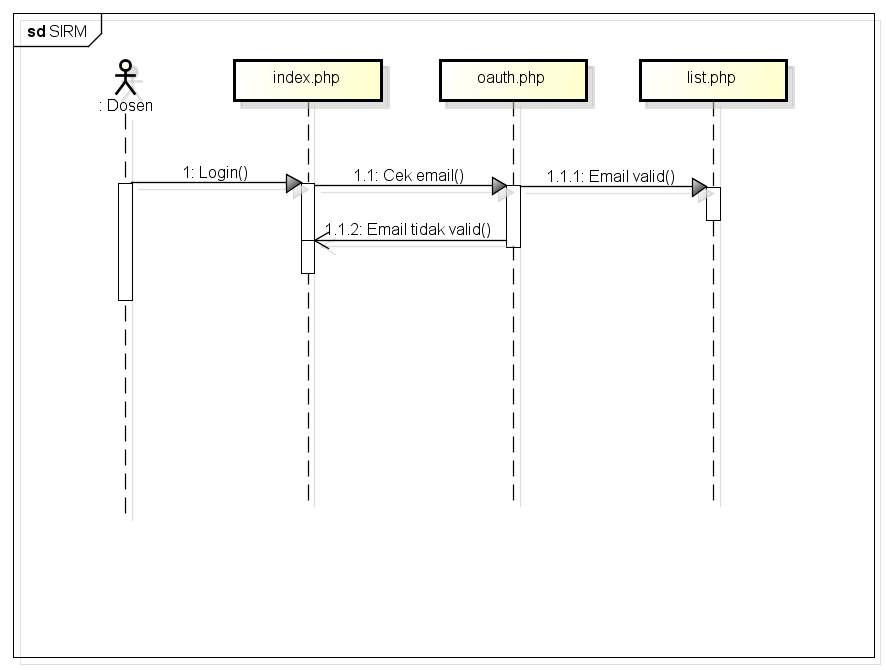
\includegraphics[scale=0.6]{Gambar/sekuenslogin.png}
%\caption[Diagram Sekuens Bagian Satu]{Diagram Sekuens Bagian Satu} 
%\label{fig:ds1}
%\end{figure}

%\begin{figure}[p]
%\centering
%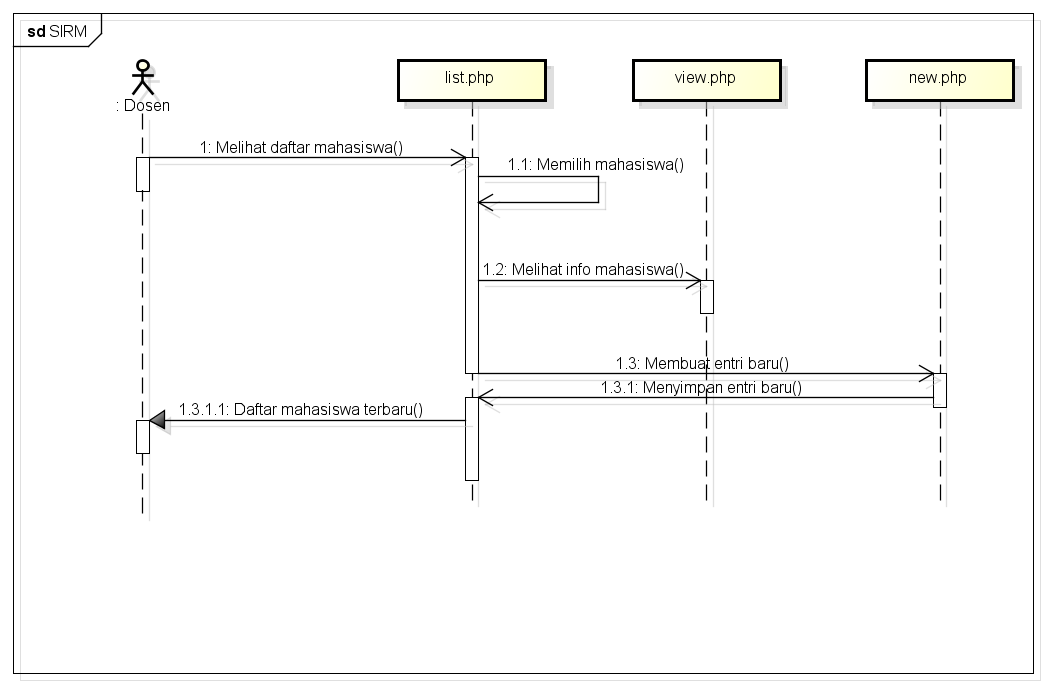
\includegraphics[scale=0.6]{Gambar/sekuenslist.png}
%\caption[Diagram Sekuens Bagian Dua]{Diagram Sekuens Bagian Dua} 
%\label{fig:ds2}
%\end{figure}

%\begin{figure}[pt]
%\centering
%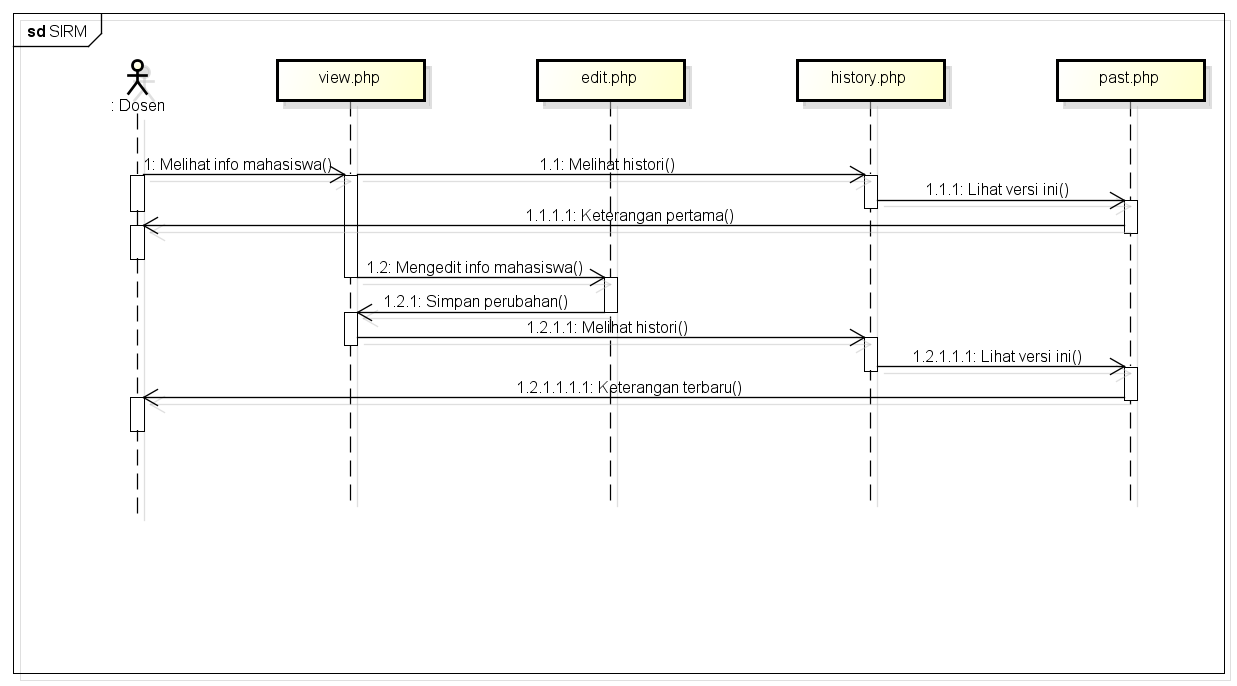
\includegraphics[scale=0.5]{Gambar/sekuensview.png}
%\caption[Diagram Sekuens Bagian Tiga]{Diagram Sekuens Bagian Tiga} 
%\label{fig:ds3}
%\end{figure}